\chapter{Ý tưởng và thuật toán}
\label{chap:algorithms}

\section{Quy hoạch động trên phân rã cây}

Ý tưởng chính là biến điều kiện thời gian thành một kiểm tra cục bộ. Khi định hướng một đường đi từ $s$ đến $z$, tại mỗi đỉnh trong $v$ chỉ cần so sánh nhãn của cạnh vào và cạnh ra:
\begin{equation}
  t_{\mathrm{in}}(v)\le t_{\mathrm{out}}(v).
  \label{eq:local-time}
\end{equation}
Chuỗi các bất đẳng thức cục bộ tương đương dãy nhãn không giảm của toàn đường đi. Với ngữ nghĩa nghiêm ngặt, dùng $<$ ở mọi đỉnh trong. Do đó, thuật toán không phải giữ toàn bộ dãy nhãn của một nghiệm bộ phận.

Cho một phân rã cây độ rộng $w$, thêm $s,z$ vào mọi túi và chuẩn hóa thành các nút lá, thêm đỉnh, thêm cạnh, quên đỉnh và ghép hai con. Mỗi cạnh nền được thêm đúng một lần; mọi túi có kích thước $b\le w+3$. Một túi là biên giữa phần đồ thị đã xử lý và phần chưa xử lý. Nghiệm bộ phận chỉ cần lưu thông tin có thể ảnh hưởng đến việc nối qua biên này.

Với mỗi đỉnh biên không phải đầu cuối, lưu một trong bốn dạng
\[
  \StateZero,\quad \StateIn(t),\quad \StateOut(t),\quad \StateBoth.
\]
$\StateZero$ nghĩa là chưa dùng cạnh; $\StateIn(t)$ và $\StateOut(t)$ nghĩa là mới có một cạnh vào hoặc ra tại hạng $t$. Khi đã có cả hai cạnh và kiểm tra thời gian thành công, trạng thái trở thành $\StateBoth$. Không cần giữ hai nhãn nữa vì đỉnh đã đủ bậc, không thể nhận thêm cạnh trong đường đi đơn.

Ngoài chữ ký bậc và nhãn $\sigma$, thuật toán lưu một phân hoạch $\Pi$ của các đỉnh biên đang được dùng. Hai đỉnh cùng khối khi chúng thuộc cùng thành phần liên thông của nghiệm bộ phận. Giá trị $F_x(\sigma,\Pi)$ tại nút phân rã $x$ là số cách chọn cạnh, hướng và nhãn tạo ra trạng thái đó, không phải danh sách các đường đi.

Bất biến yêu cầu đồ thị được chọn là một rừng, mỗi đỉnh có bậc vào và bậc ra không quá một, và mọi đỉnh trong đã quên phải có đủ hai cạnh. Mọi thành phần được chọn còn phải giao với túi hiện tại; nếu một thành phần biến mất qua biên, nó không thể nối vào đường đi cuối cùng nên trạng thái bị loại. Điều kiện này ngăn các đoạn đường thừa bị đếm cùng với nghiệm chứa $s,z$.

Ở nút lá, trạng thái rỗng có giá trị $1$. Đỉnh mới thêm bắt đầu ở $\StateZero$. Khi thêm cạnh $uv$, có lựa chọn bỏ qua cạnh hoặc chọn một trong hai hướng tại mỗi $t\in L(uv)$. Chẳng hạn, thêm cạnh ra tại hạng $t$ cập nhật
\[
  \StateZero\longrightarrow\StateOut(t),\qquad
  \StateIn(a)\longrightarrow\StateBoth\ \text{nếu }a\le t.
\]
Thêm cạnh vào đối xứng, với điều kiện $t\le a$ khi ghép vào $\StateOut(a)$. Các trường hợp vượt bậc bị loại. Nếu hai đầu đã thuộc cùng thành phần thì thêm cạnh tạo chu trình và cũng bị loại; nếu không, hợp nhất các khối liên thông.

Khi quên một đỉnh trong, chỉ nhận $\StateZero$ hoặc $\StateBoth$. Nếu đỉnh là phần tử biên cuối cùng của một khối thì không được quên trạng thái đó. Tại nút ghép, hai con có cùng túi và tập cạnh đã xử lý rời nhau. Chữ ký bậc được cộng, nhãn được so sánh nếu một con cung cấp cạnh vào và con kia cung cấp cạnh ra; số cách của hai con được nhân rồi cộng vào trạng thái cha.

Kiểm tra chu trình ở nút ghép cần nhiều hơn việc so sánh phân hoạch. Xây dựng đa đồ thị hai phía $J$: mỗi thành phần ở con trái hoặc con phải là một nút; mỗi đỉnh biên được dùng ở cả hai con tạo một cạnh nối hai thành phần chứa nó. Nếu $F_1,F_2$ là hai rừng con, $c_1,c_2$ là số thành phần và $q$ là số đỉnh dùng chung, thì
\begin{equation}
  \beta(F_1\cup F_2)=q-c_1-c_2+c(J)=\beta(J),
  \label{eq:join-cycle}
\end{equation}
trong đó $\beta(H)=|E(H)|-|V(H)|+c(H)$ là hạng chu trình. Đẳng thức theo sau từ $|E(F_i)|=|V(F_i)|-c_i$ và việc các thành phần của hợp tương ứng với các thành phần của $J$. Vì vậy, chỉ chấp nhận khi $J$ là rừng. Hai cạnh song song của $J$ phải được nhận diện là một chu trình độ dài hai, dù đồ thị nền ban đầu là đơn.

Ở gốc, chỉ nhận một thành phần chứa $s,z$, trong đó $s$ có một cạnh ra và $z$ có một cạnh vào. Các bất biến buộc đối tượng được nhận là một đường đi đơn có hướng từ $s$ đến $z$; kiểm tra~\eqref{eq:local-time} bảo đảm tính thời gian. Ngược lại, mỗi đường đi thời gian xác định duy nhất lựa chọn tại nút thêm của từng cạnh, nên được nhận đúng một lần. Đây là lập luận tính đúng và không đếm trùng của quy hoạch động.

\section{Xóa nhãn đầu cuối và cận độ phức tạp}

Một đường đi từ $s$ đến $z$ không có cạnh vào $s$ hoặc cạnh ra $z$; có thể loại các lựa chọn này ngay khi thêm cạnh. Hai đầu cuối cũng không tham gia so sánh thời gian tại đỉnh trong. Nhãn của cạnh kề đầu cuối vẫn được lưu ở đầu còn lại khi cần, nhưng không cần lưu thêm một bản tại chính đầu cuối. Vì vậy, $s$ chỉ có hai trạng thái chưa dùng/đã có cạnh ra; $z$ đối xứng. Những trạng thái chỉ khác nhãn tại đầu cuối được gộp bằng cách cộng số cách.

Gọi $\Bell_b$ là số phân hoạch của $b$ phần tử. Trong mỗi túi, chỉ nhiều nhất $w+1$ đỉnh cần giữ nhãn, nên số trạng thái được chặn bởi
\begin{equation}
  S\le4(2r+2)^{w+1}\Bell_{w+3}.
  \label{eq:states}
\end{equation}
Một nút thêm cạnh xét tối đa $\bigO(rS\operatorname{poly}(w))$ thao tác; một nút ghép xét tối đa $\bigO(S^2\operatorname{poly}(w))$. Dùng $\Bell_b\le b^b$ thu được kết quả chính dưới đây.

\begin{proposition}[Đếm với độ rộng cố định]
Với phân rã cây độ rộng $w\ge1$ được cung cấp, thuật toán đếm đúng cả hai ngữ nghĩa thời gian trong
\begin{equation}
  N(r+1)^{2w+2}2^{\bigO(w\log w)}
  \label{eq:main-bound}
\end{equation}
phép toán số học, sau chuẩn hóa phân rã. Với $w=2$, cận là $\bigO(N(r+1)^6)$.
\end{proposition}

Khi $w$ cố định, $r$ và $N$ đều bị chặn bởi kích thước đầu vào tương ứng, nên đây là thời gian đa thức. Do đó, thuật toán áp dụng cho partial 2-tree với hai đầu cuối tùy ý. Đây là câu trả lời thuật toán được đề xuất trong đề tài cho vấn đề series--parallel. Kết quả thuộc XP theo $w$, không phải FPT chỉ theo $w$: số mũ của $r$ vẫn phụ thuộc độ rộng. Cận này là cận an toàn, chưa được chứng minh tối ưu.

So với DP nội bộ lưu nhãn ở cả hai đầu cuối, cận số mũ tại nút ghép giảm từ $2w+6$ xuống $2w+2$. Lọc sớm các cặp chữ ký bậc không tương thích giúp giảm số cặp ghép trong thực tế, nhưng không thay đổi cận xấu nhất. Việc chỉ giữ các bảng còn cần cho bước tiếp theo giảm số trạng thái đồng thời sống; không được suy ra rằng mọi phân rã đều chỉ cần một bảng.

\section{Tổng tiền tố trên rừng}

Trong rừng, giữa $s,z$ có nhiều nhất một đường đi tĩnh. Nếu không liên thông, đáp án là $0$; nếu có, gọi các cạnh trên đường là $e_1,\ldots,e_P$. Đặt $f_i(t)$ là số cách chọn nhãn cho $i$ cạnh đầu, kết thúc tại hạng $t$. Với ngữ nghĩa không nghiêm ngặt,
\begin{equation}
  f_1(t)=\mathbf{1}[t\in L(e_1)],\qquad
  f_i(t)=\mathbf{1}[t\in L(e_i)]\sum_{a\le t}f_{i-1}(a).
  \label{eq:forest}
\end{equation}
Không tính lại tổng trong~\eqref{eq:forest} cho từng $t$, mà quét các hạng theo thứ tự và duy trì tổng tiền tố. Chi phí lõi giảm từ $\bigO(Pr^2)$ của truy hồi trực tiếp xuống $\bigO(Pr)$. Nếu danh sách nhãn thưa và đã sắp, quét hai danh sách liên tiếp cho cận $\bigO(P+M_P)$. Với ngữ nghĩa nghiêm ngặt, dùng tổng trên $a<t$.

Mọi cách gán nhãn hợp lệ có duy nhất nhãn cuối cùng và tiền tố trước đó, nên công thức vừa đầy đủ vừa không đếm trùng. Cận trên là cho phần đếm sau khi tìm tuyến và chuẩn bị nhãn; không bao gồm toàn bộ chi phí đọc đồ thị, tìm đường hoặc sắp xếp. Tổng tiền tố là kỹ thuật chuẩn, được dùng ở đây để cải thiện truy hồi, không phải một đóng góp lý thuyết độc lập ngang với kết quả phân rã cây.

\section{Quét sự kiện trên TTSP và cactus}

Một đối chứng tự nhiên cho TTSP lưu ma trận truyền thời gian tại mỗi thành phần. Ghép song song tương ứng phép cộng, ghép nối tiếp tương ứng phép nhân ma trận; cách trực tiếp có cận $\bigO(mr^3)$ phép toán số học và $\bigO(mr^2)$ ô số nguyên. Đây là đối chứng xây dựng trong dự án, không phải thuật toán TTSP đã công bố trong bài báo gốc.

Thuật toán chuyên biệt khai thác việc một biểu thức TTSP hợp lệ có thể định hướng từ cực $s$ đến cực $z$ thành đồ thị có hướng không chu trình. Quy nạp theo hai phép ghép cho thấy các đường đi cực--cực vô hướng tương ứng một-một với các đường đi có hướng; mọi đường đi có hướng trong đồ thị không chu trình là đơn. Nhờ đó không cần lưu riêng các lựa chọn tuyến trong ma trận.

Với cạnh thời gian có hướng $e=(u,v,t)$, đặt $D[e]$ là số tiền tố kết thúc bằng đúng cạnh đó. Duyệt đỉnh theo thứ tự tô-pô. Tại một đỉnh $v$, duy trì tổng $A$ của các tiền tố đến hợp lệ, khởi tạo $A=1$ nếu $v=s$ và $0$ nếu không. Một sự kiện cạnh vào cập nhật $A\leftarrow A+D[e]$; một sự kiện cạnh ra nhận $D[e]\leftarrow A$. Sau mọi sự kiện vào ở $z$, $A$ là đáp án.

Với các sự kiện cùng thời điểm, ngữ nghĩa không nghiêm ngặt xử lý nhóm vào trước nhóm ra; ngữ nghĩa nghiêm ngặt xử lý nhóm ra trước nhóm vào. Khi đến lượt đỉnh $v$, mọi $D[e]$ ở cạnh vào đã được tính ở đỉnh trước trong thứ tự tô-pô. Tổng $A$ do đó đúng bằng số tiền tố thỏa ngưỡng hiện tại; nối với một cạnh ra xác định duy nhất đường đi mới.

Sau nén hạng và khi định hướng hợp lệ được cung cấp, có thể sắp $2M$ sự kiện theo hạng trong $\bigO(M+r)$ và duyệt đồ thị trong $\bigO(n+m)$. Lõi đếm có cận $\bigO(n+m+M+r)$, gồm đúng $M$ phép cộng số đếm, không có phép nhân số đếm. Cận này không phải tuyên bố toàn bộ chương trình tuyến tính: sắp và nén nhãn tùy ý có thể cần $\bigO(M\log M)$; chi phí xác thực phân rã cũng phải tính riêng.

Với cactus, dùng phân rã khối bằng tìm kiếm theo chiều sâu~\cite{tarjan1972}, rồi lấy tuyến duy nhất giữa hai đầu cuối trong cây khối--đỉnh khớp. Đường đi đơn không thể ghé một khối ngoài tuyến rồi quay lại vì sẽ lặp đỉnh khớp. Trong khối cạnh, hướng từ điểm vào đến điểm ra; trong khối chu trình, hướng cả hai cung đơn theo chiều đó. Các khối nối tiếp tạo một đồ thị có hướng không chu trình bảo toàn tập nghiệm, nên áp dụng cùng phép quét sự kiện cho hai đầu cuối tùy ý.

\section{Giới hạn cấu trúc và chi phí số lớn}

Không thể thay phương pháp phân rã cây bằng phép định hướng sự kiện cho mọi đồ thị độ rộng hai. Trong đồ thị Wheatstone ở Hình~\ref{fig:wheatstone}, hai đường $s-u-v-z$ và $s-v-u-z$ cần hai hướng trái ngược của cạnh $uv$. Một định hướng duy nhất không thể giữ cả hai nghiệm. Tương tự, định hướng TTSP theo hai cực cũ có thể làm mất các đường đi của truy vấn nội bộ. Đây là lý do vẫn cần DP tổng quát.

\begin{figure}[htbp]{Đồ thị Wheatstone có treewidth hai. Hai đường đi được nêu trong nội dung cần hai hướng ngược nhau của cạnh giữa $u,v$.}
\label{fig:wheatstone}
\centering
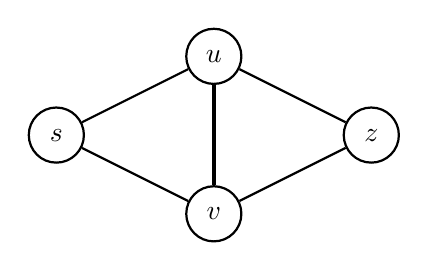
\begin{tikzpicture}[every node/.style={circle,draw,minimum size=7mm,inner sep=1pt},line width=0.8pt]
  \node (s) at (0,0) {$s$};
  \node (u) at (2,1) {$u$};
  \node (v) at (2,-1) {$v$};
  \node (z) at (4,0) {$z$};
  \draw (s)--(u)--(z) (s)--(v)--(z);
  \draw[line width=1.4pt] (u)--(v);
\end{tikzpicture}
\end{figure}

Các cận trước đếm phép toán số học. Số đường đi có thể vượt 64 bit, nên cần tính thêm chi phí số nguyên lớn. Đặt $B$ là số bit lớn nhất của mọi số đếm trung gian. Một cận an toàn là $B=\bigO(m\log(1+2r))$, vì mỗi cạnh nền có thể bị bỏ qua hoặc được chọn với một trong hai hướng và tối đa $r$ nhãn. Với phép cộng tuyến tính và phép nhân dài thông thường, DP có cận bit bằng~\eqref{eq:main-bound} nhân thêm $\bigO(B^2)$; quét sự kiện có cận $\bigO((n+m+M+r)B)$. Như vậy, tính đa thức khi $w$ cố định vẫn được bảo toàn trong mô hình bit, không dựa vào giả định số nguyên lớn là miễn phí.
